\documentclass[xetex,table]{beamer}

\usepackage[autostyle]{csquotes}
\usepackage{hyperref}
\usepackage{color}
\usepackage{setspace}
\usepackage{listings}
\usepackage{minted}

\usetheme{metropolis}

\usemintedstyle{perldoc}

\title{Buildroot}
\subtitle{Making Embedded Linux Easy}
\author{Luca Ceresoli\\
  \href{mailto:luca@lucaceresoli.net}{luca@lucaceresoli.net}\\
  \url{http://lucaceresoli.net}
}
\date{Linux Day 2018\\
  BgLUG}

\begin{document}

\maketitle

\begin{frame}{Agenda}
  \begin{itemize}
  \item Introduzione
  \item Buildroot
  \item Packages
  \item Conclusioni
  \end{itemize}
\end{frame}

\section{Introduzione}

\begin{frame}{Che cosa è un sistema embedded}
  \begin{itemize}
    \pause\item È un computer
    \begin{itemize}
      \pause\item {\color{red} incorporato} in un sistema
      \pause\item programmato per {\color{blue} una specifica applicazione}
      \pause\item con una piattaforma {\color[rgb]{0,0.5,0} hardware ad hoc}
    \end{itemize}
  \item[] {\tiny(\url{https://it.wikipedia.org/wiki/Sistema_embedded})}
    \pause\item Esempi
    \begin{itemize}
      \pause\item Router ADSL
      \pause\item TV
      \pause\item Stampante 3D
      \pause\item Macchina tessile
      \pause\item Videocitofono
      \pause\item Autoradio
      \pause\item\dots
    \end{itemize}
  \end{itemize}
\end{frame}

\begin{frame}{Sistemi embedded}
  \center\includegraphics[width=1.0\textwidth]{images/embedded-systems-range.pdf}
\end{frame}

\begin{frame}{Anatomia di un Sistema Operativo}
  \center\includegraphics[width=1.0\textwidth]{images/operating-system.pdf}
\end{frame}

\begin{frame}{Host VS Target}
  \center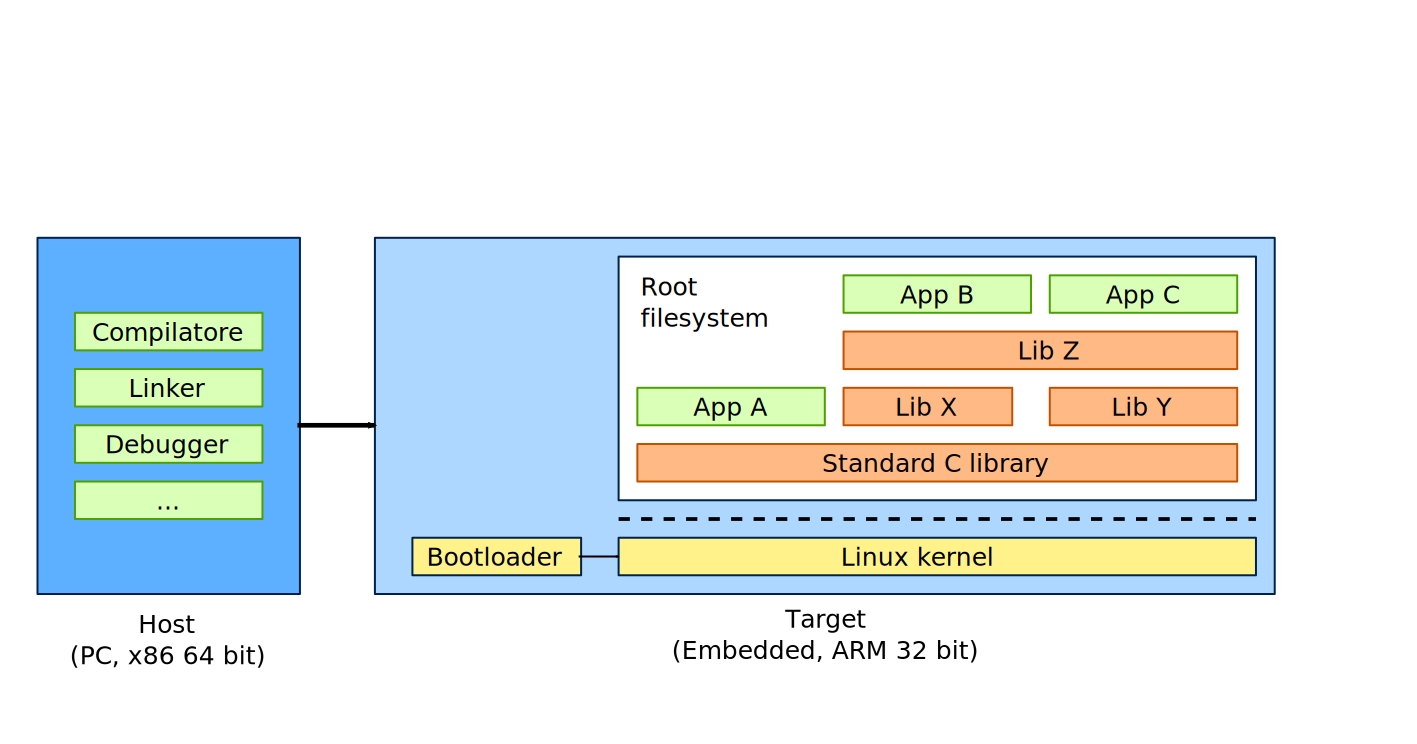
\includegraphics[width=1.0\textwidth]{images/host-target.pdf}
\end{frame}

\begin{frame}{Buildsystem}
  \center\includegraphics[width=1.0\textwidth]{images/in-br-out.pdf}
\end{frame}

\begin{frame}[standout]
  Demo: la prima build
\end{frame}

\begin{frame}{BeagleBone Black}
  \begin{columns}
    \column{0.35\textwidth}
    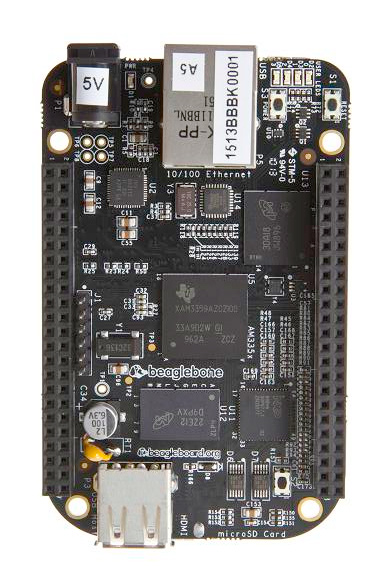
\includegraphics[width=\textwidth]{images/Beaglebone_Black.jpg}
    {\tiny
      \url{https://beagleboard.org/black}\\
      CC BY-SA 3.0}
    \column{0.65\textwidth}
    \begin{itemize}
    \item SoC: AM3358/9
    \item Core: ARM Cortex-A8 32-bit 1 GHz
    \item RAM: to 512 MB
    \item Storage: 4GB eMMC
    \item \url{https://beagleboard.org/black}
    \item \url{https://en.wikipedia.org/wiki/BeagleBoard\#BeagleBone_Black}
    \end{itemize}
  \end{columns}
\end{frame}

\section{Buildroot}

\begin{frame}{Buildroot}
  \begin{itemize}
  \item Buildroot --- Making Embedded Linux Easy
  \pause\item Strumento per generare tutti i componenti
    \begin{itemize}
    \item Cross-toolchain
    \item Bootloader
    \item Kernel
    \item Root filesystem: librerie, applicativi\ldots
      \begin{itemize}
      \item Contiene le ``ricette'' per compilare 2300+ pacchetti
      \end{itemize}
    \item File ``immagine'' da scrivere in flash, SD\ldots
    \end{itemize}
  \pause\item Obiettivi
    \begin{itemize}
    \item Semplice da usare, capire, adattare
    \item Snello, veloce, efficiente
    \end{itemize}
  \pause\item Community project
  \pause\item \url{http://buildroot.org/}
  \end{itemize}
\end{frame}

\begin{frame}{Fondamenta di Buildroot}
  \center\includegraphics[width=0.8\textwidth]{images/br-tools.pdf}
\end{frame}

\begin{frame}{Configurazione}
  \begin{columns}
    \column{0.8\textwidth}
    \begin{itemize}
    \item Configurazione = {\em cosa} vogliamo che Buildroot produca
    \onslide<2->{
      \item Buildroot di configura con {\tt Kconfig}
        \begin{itemize}
        \item Il sistema di configurazione del kernel
        \end{itemize}
    }
    \onslide<3->{
      \item Parametri configurabili
        \begin{itemize}
        \item Tipo di processore
        \item Toolchain
        \item Bootloader
        \item Kernel
        \item Pacchetti da installare
        \item Tipi di root filesystem
        \item Opzioni di compilazione
        \item Configurazione del sistema
        \end{itemize}
    }
    \end{itemize}
    \column{0.2\textwidth}
    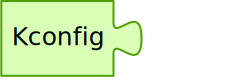
\includegraphics[width=\textwidth]{images/br-tools-kconfig.pdf}
  \end{columns}
\end {frame}

\begin{frame}{Configurazione}
  \begin{columns}
    \column{0.8\textwidth}
    \begin{itemize}
    \item Utilizzo
      \begin{itemize}
      \item {\tt make help}
      \item {\tt make list-defconfigs}
      \item {\tt make <similar\_board>\_defconfig}
      \item {\tt make menuconfig}      
      \end{itemize}
    \item La configurazione si trova in {\tt .config}
      \begin{itemize}
      \item {\tt make savedefconfig} --- salva in forma compatta
      \end{itemize}
    \end{itemize}
    \column{0.2\textwidth}
    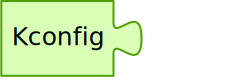
\includegraphics[width=\textwidth]{images/br-tools-kconfig.pdf}
  \end{columns}
\end {frame}

\begin{frame}{Build}
  \begin{columns}
    \column{0.8\textwidth}
    \begin{itemize}
      \item Build = produzione di kernel, rootfs etc a partire dai
        sorgenti
    \onslide<2->{
      \item Basato su {\tt Make}
        \begin{itemize}
        \item Lo strumento più usato per la compilazione di software
        \item Gestisce le dipendenze tra pacchetti
        \end{itemize}
    }
    \end{itemize}
    \column{0.2\textwidth}
    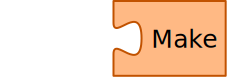
\includegraphics[width=\textwidth]{images/br-tools-make.pdf}
  \end{columns}
\end{frame}

\begin{frame}{Elementi della build}
  \center\includegraphics[width=0.8\textwidth]{images/dependencies2.pdf}
\end{frame}

\begin{frame}{Build steps}
  \begin{itemize}
  \item Per ciascun pacchetto vengono eseguiti diversi passi:
    \begin{itemize}
    \item Source (download dei sorgenti)
    \item Extract
    \item Patch
    \item Configure
    \item Build
    \item Install
    \end{itemize}
  \end{itemize}
\end{frame}

\begin{frame}[standout]
  Demo: boot!
\end{frame}

\begin{frame}[standout]
  Demo: analisi dell'output
\end{frame}

\section{Packages}

\begin{frame}[fragile]{Un pacchetto semplice}
  \begin{minted}[frame=single,autogobble,fontsize=\footnotesize]{text}
    buildroot
    `-- package
        `-- netcat
            +-- Config.in
            +-- netcat.mk
            +-- netcat.hash
            `-- 0001-signed-bit-counting.patch
  \end{minted}
\end{frame}

\begin{frame}[fragile]{\tt Config.in}

  {\tt package/netcat/Config.in}
  \begin{minted}[frame=single,autogobble,fontsize=\footnotesize]{Kconfig}
    config BR2_PACKAGE_NETCAT
        bool "netcat"
        depends on BR2_PACKAGE_BUSYBOX_SHOW_OTHERS
        help
          Netcat is a featured networking utility which reads and
          writes data across network connections, using the TCP/IP
          protocol.
          [...]

          http://netcat.sourceforge.net/download.php
  \end{minted}
\end{frame}

\begin{frame}[fragile]{\tt netcat.mk}

  {\tt package/netcat/netcat.mk}
  \begin{minted}[frame=single,autogobble,fontsize=\footnotesize]{makefile}
    NETCAT_VERSION = 0.7.1
    NETCAT_SITE = http://downloads.sourceforge.net/project \
                        /netcat/netcat/$(NETCAT_VERSION)
    NETCAT_LICENSE = GPL-2.0+
    NETCAT_LICENSE_FILES = COPYING

    $(eval $(autotools-package))
  \end{minted}
\end{frame}

\begin{frame}[fragile]{\tt netcat.hash}

  {\tt package/netcat/netcat.hash}
  \begin{minted}[frame=single,autogobble,fontsize=\footnotesize]{text}
  # Locally computed:
  sha256  30719c9a4ffbcf1...0c68a066f  netcat-0.7.1.tar.gz
  \end{minted}
\end{frame}

\begin{frame}[fragile]{Patches}
  \begin{minted}[frame=single,autogobble,fontsize=\footnotesize]{text}
buildroot
`-- package
    `-- netcat
        +-- Config.in
        +-- netcat.mk
        +-- netcat.hash
        `-- 0001-signed-bit-counting.patch
  \end{minted}
  \begin{itemize}
  \item Patch = insieme di modifiche ai sorgenti del pacchetto
  \item Vengono applicate automaticamente
    \begin{itemize}
    \item nello step {\tt patch} (dopo {\tt extract})
    \end{itemize}
  \end{itemize}
\end{frame}

\begin{frame}[fragile]{Un pacchetto un po' più complesso}

  {\tt package/sl/sl.mk}
  \begin{minted}[frame=single,autogobble,fontsize=\footnotesize]{makefile}
    SL_VERSION = 5.02
    SL_SITE = $(call github,mtoyoda,sl,$(SL_VERSION))
    SL_LICENSE = Custom
    SL_LICENSE_FILES = LICENSE
    SL_DEPENDENCIES = ncurses

    define SL_BUILD_CMDS
        $(MAKE) -C $(@D) $(TARGET_CONFIGURE_OPTS)
    endef

    define SL_INSTALL_TARGET_CMDS
        $(INSTALL) -m 0755 -D $(@D)/sl $(TARGET_DIR)/usr/bin/sl
    endef

    $(eval $(generic-package))
  \end{minted}
\end{frame}

\section{Conclusioni}

\begin{frame}
  \begin{center}
    Grazie per l'attenzione!

    \vspace{0.1\textheight}

    {\Huge Domande?}

    \vspace{0.1\textheight}

    \href{mailto:luca@lucaceresoli.net}{luca@lucaceresoli.net}\\
    \url{http://lucaceresoli.net}

    \textcopyright{} Copyright 2018, Luca Ceresoli\\

    \vspace{0.2\textheight}

    \tiny
    Materiale rilasciato sotto licenza\\
    Creative Commons Attribution - Share Alike 3.0 \\
    \url{https://creativecommons.org/licenses/by-sa/3.0/} \\
\end{center}
\end{frame}

\end{document}
